\documentclass[12pt,a4paper]{article}
\usepackage{solutions}
\usepackage{multicol}
\usepackage{float}

\title{Домашнее задание от 28.09.\\Теоретическая информатика. 2 курс.\\Решения.}
\author{Глеб Минаев @ 204 (20.Б04-мкн)}
% \date{}

\newcommand{\Id}{\mathrm{Id}}

\begin{document}
    \maketitle

    \begin{multicols}{2}
        \tableofcontents
    \end{multicols}

    \begin{problem*}[2.3]
        Для всякого $p \geqslant 1$ можно взять слово $w := a^p b^p \in L$, и тогда для всякого разбиения $w = xyz$, где $|xy| \leqslant p$ и $y \neq \varepsilon$, верно что $x = a^k$, $y = a^l$, $z = a^{p-k-l} b^p$, а значит для всякого $m \geqslant 2$
        \[x y^m z = a^{k + ml + (p-k-l)} b^p = a^{p + (m-1)l} b^p \notin L.\]
        Получаем прямое противоречие с леммой о накачке.
    \end{problem*}

    \begin{problem*}[2.4]\ 
        \begin{figure}[H]
            \centering
            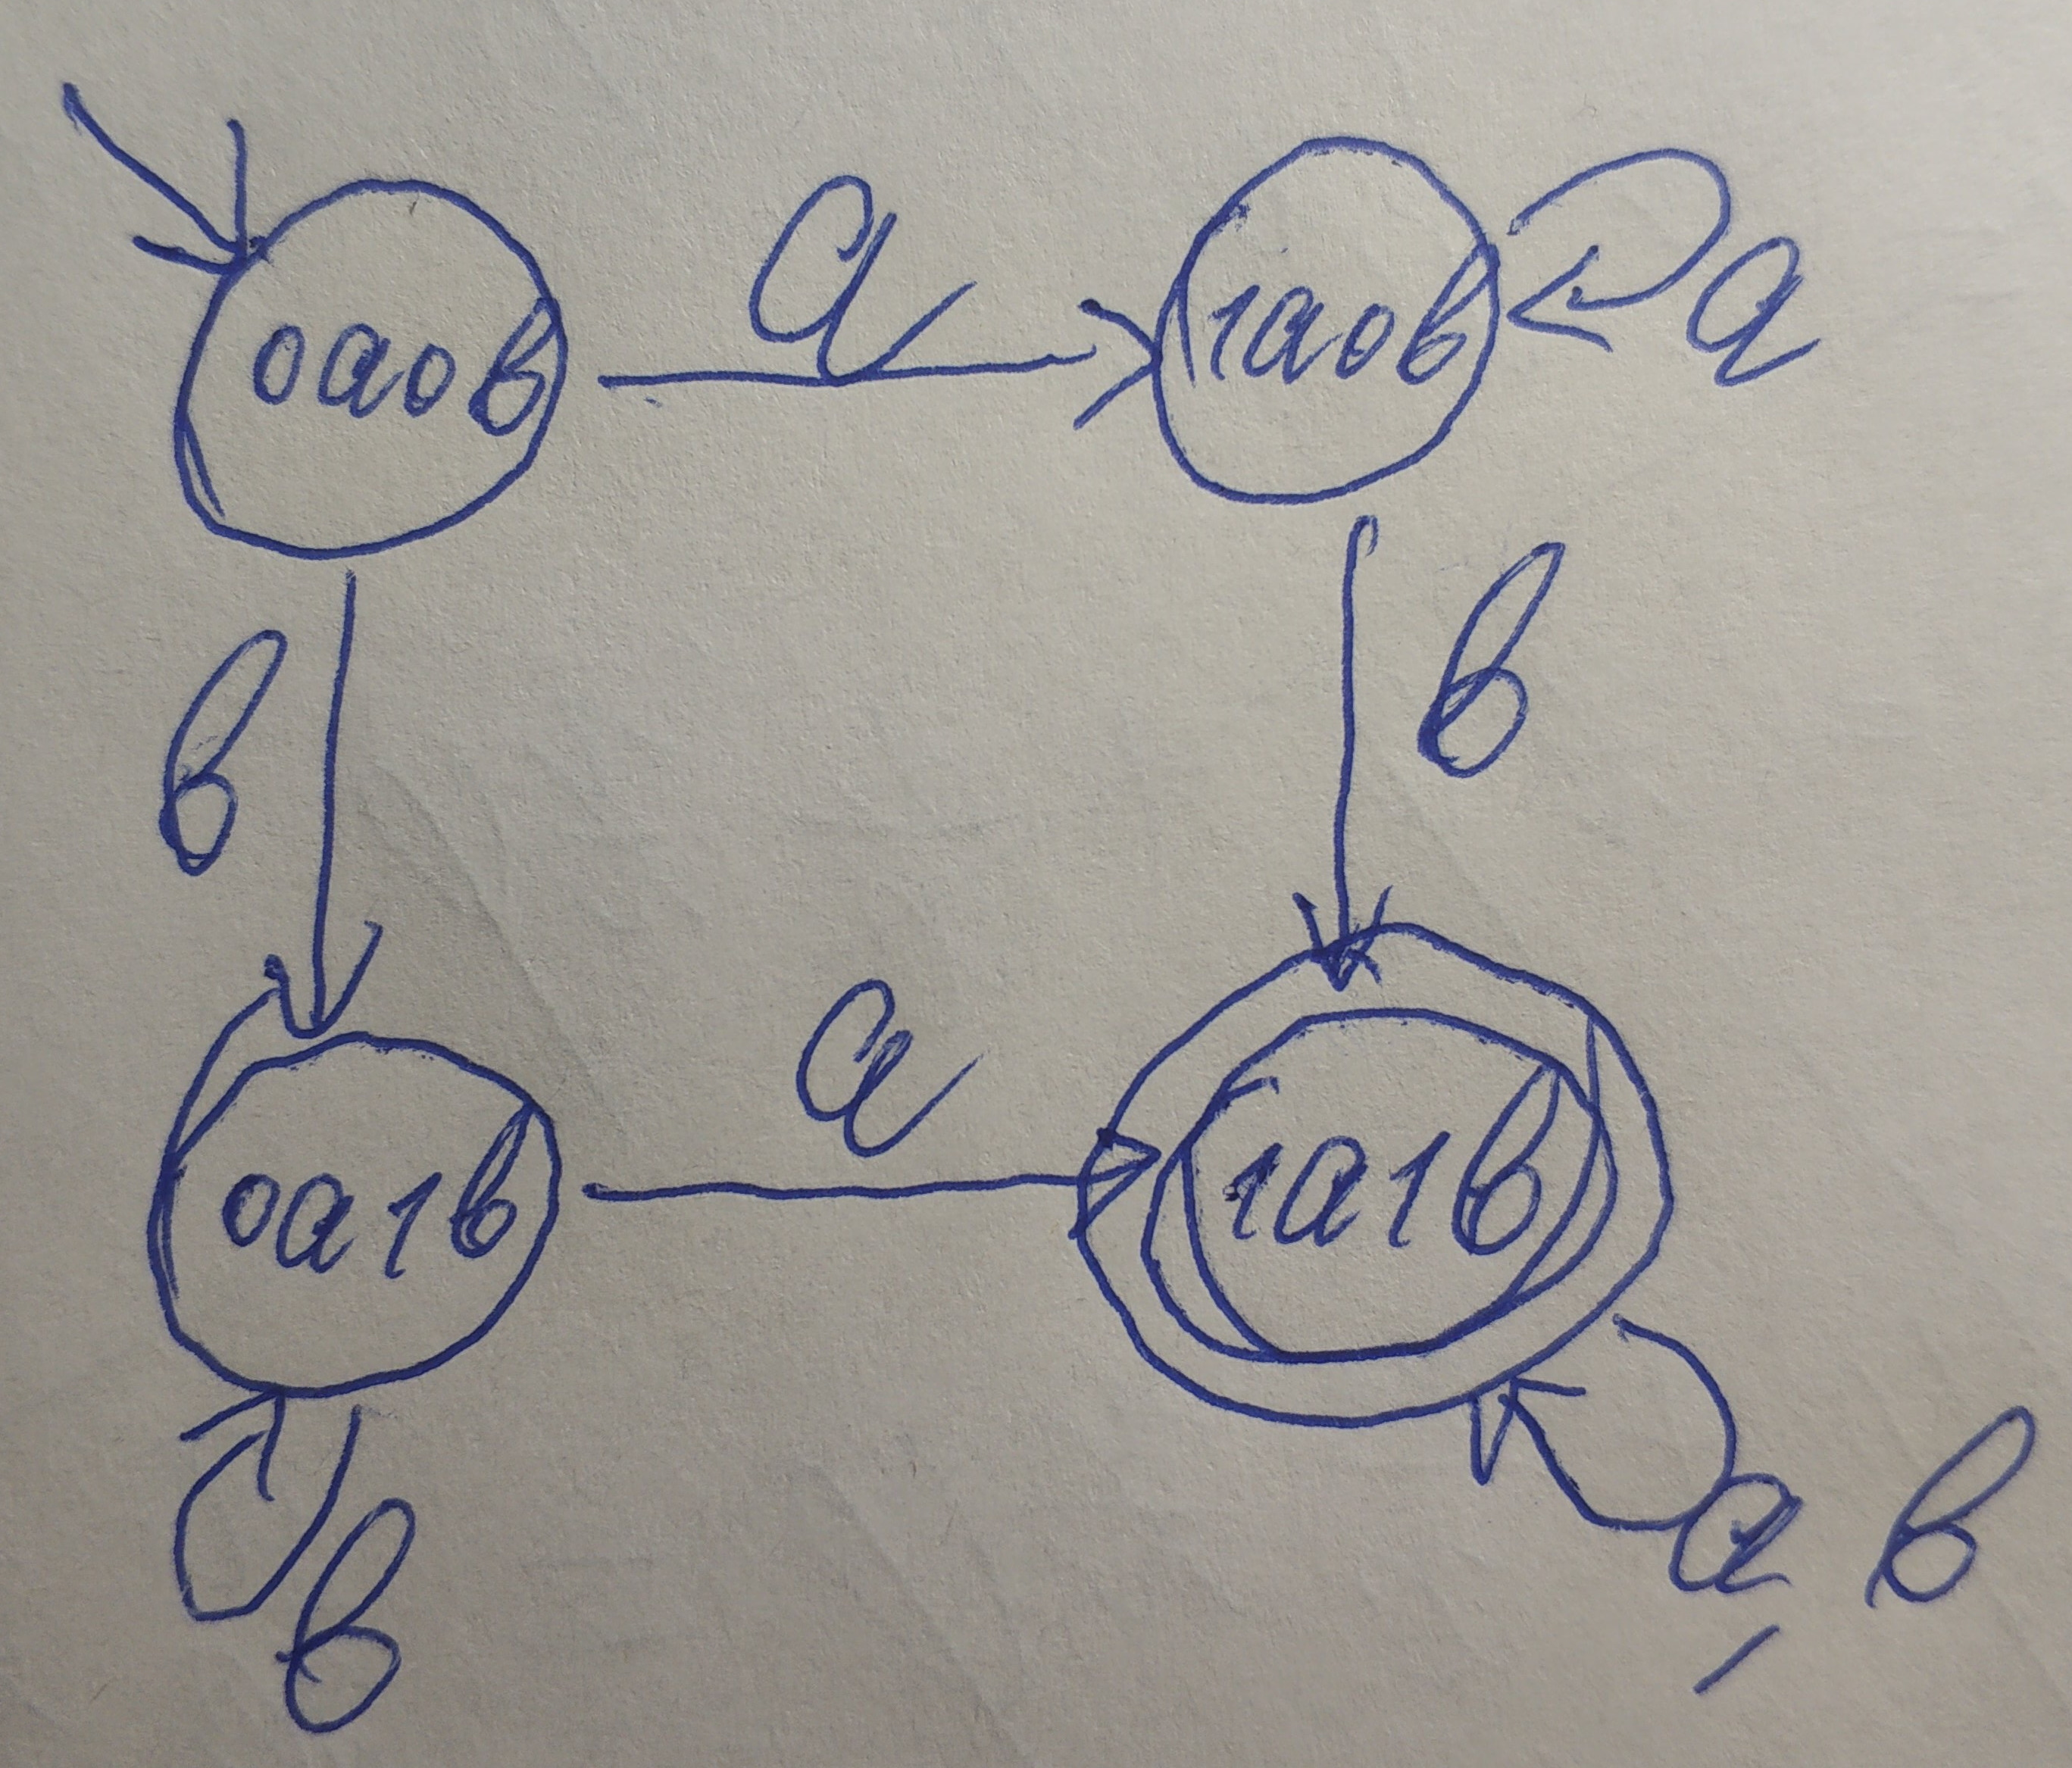
\includegraphics[height=5cm]{TI-HW-004-1.jpg}
        \end{figure}
    \end{problem*}

    \begin{problem*}[2.5]
        Для всякого $p \geqslant 1$ можно взять слово $w := a^p b^{p! + p} \in L$, и тогда для всякого разбиения $w = xyz$, где $|xy| \leqslant p$ и $y \neq \varepsilon$, верно что $x = a^k$, $y = a^l$, $z = a^{p-k-l} b^{p! + p}$, а значит есть $m = \frac{p!+l}{l}$, что $k + ml + (p-k-l) = p!+p$, а тогда
        \[x y^m z = a^{k + ml + (p-k-l)} b^{p! + p} = a^{p! + p} b^{p! + p} \notin L.\]
        Получаем прямое противоречие с леммой о накачке.
    \end{problem*}

    \begin{problem*}[4.2]
        Пусть ДКА $A = (\Sigma, Q, q_0, \delta, F)$ реализует язык $L$. Рассмотрим ДКА
        \[B := (\Sigma, Q^Q, f_0 := \Id_Q, \eta, \{f \in Q^Q \mid \exists i \geqslant 2 \colon \; f^i(q_0) \in F\}),\]
        где
        \[\eta(f, a) := \delta_a \circ f.\]
        Тогда несложно видеть, что $\eta(f_0, w) = \delta^*_w$, а тогда $w$ принимается тогда и только тогда, когда есть $i \geqslant 2$, что $(\delta^*_w)^i(q_0) \in L$, т.е. $\delta(q_0, w^i) \in L$, т.е. $w_i \in L$. Таким образом
        \[L(B) = E(L).\]
    \end{problem*}

    \begin{problem*}[4.3]
        Пусть $L = \Sigma^*$ --- очевидно, регулярный. Тогда $\mathrm{PAL}(L)$ --- язык всех палиндромов --- не регулярен (задача 2.1).
    \end{problem*}

    \begin{problem*}[4.4]
        Пусть ДКА $A = (\Sigma, Q, q_0, \delta, F)$ реализует язык $L$. Рассмотрим НКА
        \[B := (\Sigma, Q^Q \cup Q \times Q^Q, f_0 := \Id_Q, \eta, \{(q, f) \in Q \times Q^Q \mid f(q) \in F\}),\]
        где
        \[
            \eta(t, a) :=
            \begin{cases}
                \{\delta_a \circ t; (q_0, \delta_a \circ t)\}& \text{ если } t \in Q^Q,\\
                \{(\delta(q, a), f)\}& \text{ если } t = (q, f) \in Q \times Q^Q.\\
            \end{cases}
        \]
        Тогда несложно показать по индукции, что $\eta^*(f_0, w)$ --- множество, состоящее из $\delta_w$ и пар $(\delta(q_0, u), \delta_v)$ для каждого разбиения $w = vu$. А тогда $w$ принимается тогда и только тогда, когда есть разбиение $w = vu$, что $\delta_v(\delta(q_0, u)) \in L$, т.е. $\delta(\delta(q_0, u), v) \in L$, т.е. $\delta(q_0, uv) \in L$. Таким образом
        \[L(B) = \mathrm{SHIFT}(L).\]
    \end{problem*}

    \begin{problem*}[4.5]
        Пусть ДКА $A = (\Sigma, Q, q_0, \delta, F)$ реализует язык $L$. Рассмотрим ДКА
        \[B := (\Sigma, Q \times 2^Q, (q_0; F), \eta, \{(q; S) \in Q \times 2^Q \mid q \in S\}),\]
        где
        \[\eta((q, S), a) := (\delta(q, a), \{p \in Q \mid \exists s \in \Sigma^2 \colon\; \delta(p, s) \in S\}).\]
        Тогда несложно видеть, что $\eta(q_0, w) = (\delta(q_0, w), S)$, где $S$ --- множество состояний, из которых можно попасть хоть как-нибудь в $F$ за ровно $|w|$ переходов. А тогда $w$ принимается тогда и только тогда, когда есть $v \in \Sigma^{2|w|}$, что $\delta(q_0, wv) \in F$. Таким образом
        \[L(B) = 1/3(L).\]
    \end{problem*}

    \begin{problem*}[5.1]\ 
        \begin{figure}[H]
            \centering
            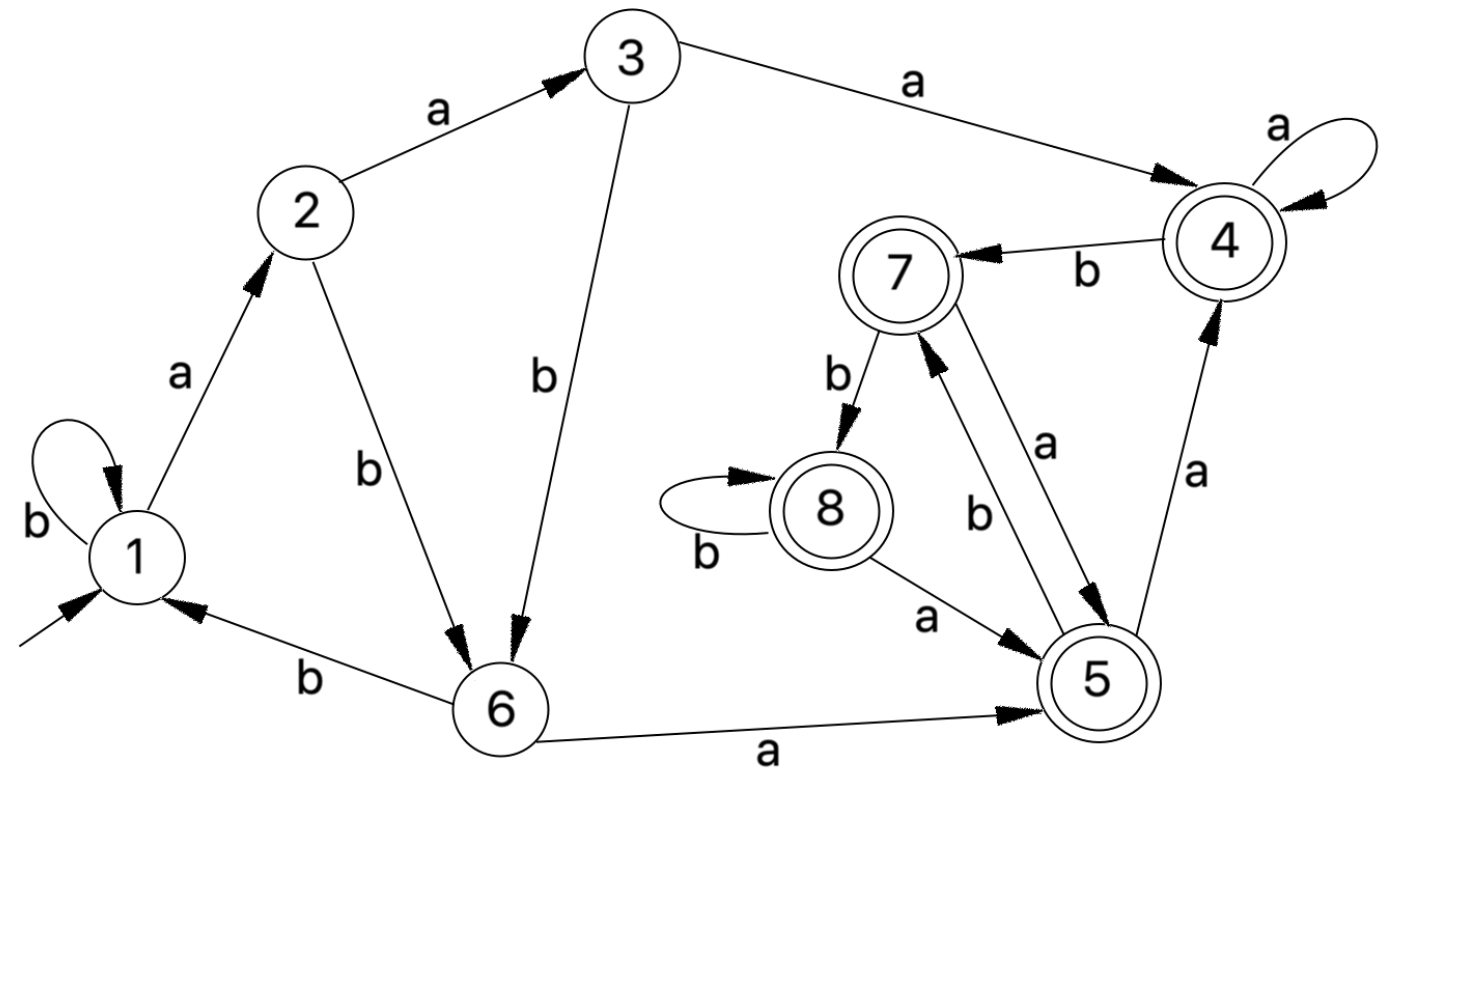
\includegraphics[height=5cm]{TI-HW-004-2.png}
        \end{figure}
        Будем использовать нумерацию рисунка. Тогда мы имеем последовательность разбиений:
        \begin{gather*}
            \{\{1; 2; 3; 6\}; \{4; 5; 7; 8\}\}
            \intertext{\centering ($1$ и $2$ имеют стрелки $a$ и $b$ в первое множество, а $3$ и $6$ --- стрелку $a$ во второе, $b$ в первое)}
            \{\{1; 2\}; \{3; 6\}; \{4; 5; 7; 8\}\}
            \intertext{\centering ($3$ имеет стрелку $b$ во второе множество, а $6$ --- в третье)}
            \{\{1; 2\}; \{3\}; \{6\}; \{4; 5; 7; 8\}\}
            \intertext{\centering ($1$ имеет стрелку $a$ в первое множество, а $2$ --- нет)}
            \{\{1\}; \{2\}; \{3\}; \{6\}; \{4; 5; 7; 8\}\}
            \intertext{\centering (первые четыре множества неделимы, а последнее имеет стрелки в себя, поэтому тоже неделимо).}
        \end{gather*}
        Итого нужно просто склеить все принимающие состояния в одно.
    \end{problem*}
\end{document}